\chapter{Design}
	This chapter describes the initial design of the software, that is the design thought by the team at the beginning of the development.
	For reasons of clarity, the description of the architecture follows a top-down approach and makes use of diagrams. 		The first section gives an overview of the software and the others study in deep specific aspects of it.

%	\section{How to read the chapter}
	To better explain the contents and the structure of the design, the description is supported by \mbox{UML} diagrams. The following sections describe the software at different levels of detail and the diagrams reflect this approach. In the first section, for example, they are used only to present how the classes are organized in the overall structure and for this contain only the names of the classes. Further details are added in the diagrams in the next sections, according with the top-down approach of the chapter.

\begin{comment}
	As the chosen development process is incremental and iterative as described in chapter \ref{devProcChap}, the initial design represents a reference in which are described only the well known aspects of the project. According to the agile development, the team chose to postpone the design of specific features of the software not well defined a-priori. This explains why the description does not enters into details. 
\end{comment}
	As described in chapter \ref{devProcChap}, the chosen development process is incremental and iterative.
	According to this choice, the initial design represents a reference in which are described only the well known aspects of the project. The choices regarding specific features not well defined a-priori are demanded. For this reason in this chapter the description, although it deepens specific topics, does not enter into detail. 
		
	The reader will notice that some classes that appear in the following diagrams are not described in the chapter. The reason of this is that they do not accomplish to any functions described in the requirements section of \mbox{chapter \ref{chObjective}}. Their presence makes sense in the context of the whole software, described in \ref{futureDev}. It has been decided not to remove such classes from the diagrams because they influence the project and motivate particular design and implementation choices.

\begin{comment}
The classes \emph{MarkerDetector} and \emph{QRScanner} do not accomplish to the communication with ACT-R nor the extraction of features in the way it is defined in the requirements section of chapter \ref{chObjective}. Their presence makes sense in the context of the whole software, described in \ref{futureDev}. Both of these classes work on video streams: MarkerDetector data looks for \emph{markers}, images with pre-determined patterns, and QRScanner searches for \mbox{QR} elements and tries to decode them. Both marker and \mbox{QR} elements are considered features. This fact explains the presence of these two classes in the feature extraction process. It has been decided not to remove them from the diagrams because they influence the design of the software and represent the motivations to particular design and implementation choices.
\end{comment}

\begin{comment}
	Moreover, as the software has been developed in team but this document focuses only on a subset of the whole work, some classes are shown in the diagrams but are not described. The team developed them in order to accomplish tasks fundamental in the whole context of the software but not of interest in this particular work. Such classes can not be removed from the diagrams because they influence the design.
\end{comment}

	\section{Overview of the design}
	The software is composed of four main parts, one for processing images and videos, one for containing the hierarchy of the objects recognized during such processing, one for allowing ACT-R to communicate with the software and one containing all the utility functions used by all the other parts.

	\begin{figure}[h]
	  \begin{center} 
	    \fbox{	
	       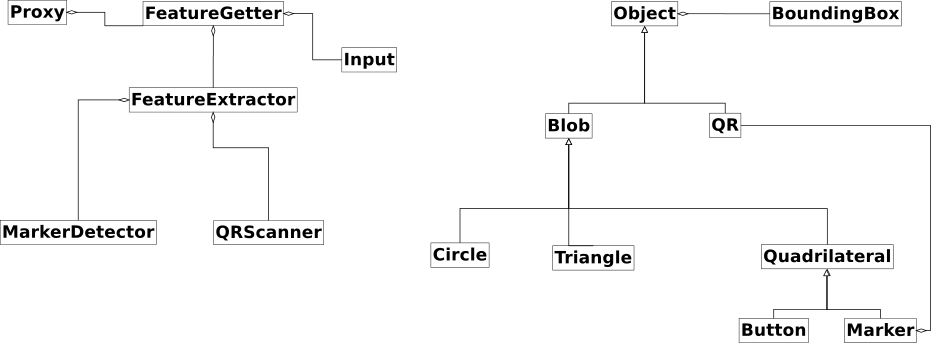
\includegraphics[scale=0.55]{images/ch_05/progettazione_overview.png}
	    }
	  \end{center} 
	  \caption{\textit{Class diagram illustrating a high level overview of the designed parts of the software}}  
	  \label{fig:swArchitecture}
 	\end{figure}		

	Image \ref{fig:swArchitecture} shows a class diagram which describes two of the parts that compose the software. 
	The part dedicated to the processing of images and video is located on the left and is composed by the classes \emph{Proxy}, \emph{FeatureGetter}, \emph{FeatureExtractor}, \emph{Input}, \emph{MarkerDetector} and \emph{QRScanner}.
	The object hierarchy, which is shown on the right, contains the classes \emph{Object}, \emph{BoundingBox}, \emph{Blob}, \emph{QR}, \emph{Circle}, \emph{Triangle}, \emph{Quadrilateral}, \emph{Button} and \emph{Marker}.

	

	The other two parts are not included in the design diagrams for different reasons. 
	According to the non-functional requirements, the team planned to try different solutions in order to implement the communication between the software and ACT-R. As different approaches can lead to different architectures, this part has not been designed a priori.
	Regarding the utility part, it depends strongly by the future design and implementations choices and is influenced by the chosen communication technique. These factor leads it to be very instable and volatile. 
	For these reasons and according to the agile development, the team decided not to spend time in planning a fixed structure for it at the beginning.

\begin{comment}
	Regarding the utility part, as it depends strongly by the implementations choices, it is very instable and volatile. Moreover, it is influenced by the chosen communication technique, which, as just described, has not been planned.
	For these reasons, according to the agile development the team decided not to spend time in planning a fixed structure for it.
\end{comment}
	
	
	\section{Feature Extraction Classes}\label{featExtraction}	
	The classes that play the role of acquiring the images and extracting features from them are \emph{Input}, \emph{FeatureGetter} and \emph{FeatureExtractor}. \emph{Proxy} has the role of intermediation between this part of the software and the one which manages the communication with \mbox{ACT-R}.

\begin{comment}
	\emph{MarkerDetector} and \emph{QRScanner} classes have been developed by the team in order to make the software locate markers and finding and decoding QR object. These tasks, although are fundamental in the whole work, are not significant in the objective of this particular work, so they are not described.
\end{comment}
	\begin{figure}[h]
	  \begin{center} 
	    \fbox{	
	       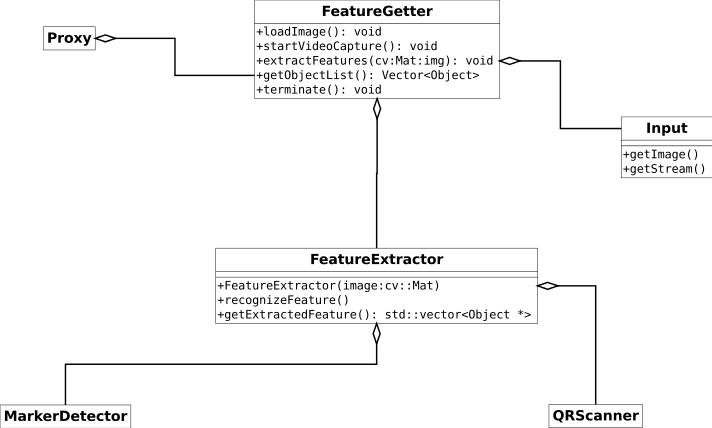
\includegraphics[scale=0.65]{images/ch_05/feature.png}
	    }
	  \end{center} 
	  \caption{\textit{Class diagram illustrating the main roles in the feature extraction process}}  
	  \label{fig:FeatureDesign}
 	\end{figure}
	
	Figure \ref{fig:FeatureDesign} contains the class diagram that designs the interface of these classes.
	\emph{FeatureExtractor} represents the core of this part. It receives in input an image and processes it in order to extract the features that contains. For each extracted feature it creates a correspondent element in the \emph{object hierarchy}. Such hierarchy is described in section \ref{classHierarchy}. Once the objects are created, the class creates a list containing all of them and delivers it to FeatureGetter. 
	FeatureExtractor is also responsible for accomplish other goals described in the requirements, like recognizing colors of pixels and objects, calculating the distances of two objects as well as the relative position of one object in respect with another one and making dimensional comparisons between two objects. These features have not been included in the initial design of the class even if it has been thought that this class would have accomplished all these tasks.

	\emph{Input} is responsible for interacting with the file system and the hardware of the computer. In particular its tasks are loading images from files, saving images to files and loading video streams from the web-cam. The acquired data are delivered to FeatureGetter. 

	\emph{FeatureGetter} represents a level of abstraction that avoids to call directly the functions of FeatureExtractor and Input, providing a simpler interface. Its functions create the Input object, receive from it the input data, delivers it to FeatureExtractor for the extraction of the features and delivers the received object list to Proxy.

	\emph{Proxy} represents a further level of abstraction between FeatureGetter and the part of the software which manages the communication with ACT-R. Most of the procedures for the communication with the artificial intelligence framework, in fact, need to use specific data types. This class has the main function to transform each object of the object list in the type necessary for the communication to ACT-R.

	For the reason explained at the beginning of the chapter, \emph{MarkerDetector} and \emph{QRScanner} are not described in this work.

\begin{comment}
	The classes \emph{MarkerDetector} and \emph{QRScanner} do not accomplish to the communication with ACT-R nor the extraction of features in the way it is defined in the requirements section of chapter \ref{chObjective}. Their presence makes sense in the context of the whole software, described in \ref{futureDev}. Both of these classes work on video streams: MarkerDetector data looks for \emph{markers}, images with pre-determined patterns, and QRScanner searches for \mbox{QR} elements and tries to decode them. Both marker and \mbox{QR} elements are considered features. This fact explains the presence of these two classes in the feature extraction process. It has been decided not to remove them from the diagrams because they influence the design of the software and represent the motivations to particular design and implementation choices.
\end{comment} 		

\begin{comment}
In this way it represents the only way in which the both It provides functions to load images, extract features from them and return a list of \emph{Object}, each of which represents one of the detected feature. 
The objects are elements of the object hierarchy, that is described in \ref{classHierarchy}. The class also allows to load a video from a webcam, extract a frame from it and apply the same algorithms to it in order to apply the feature extractions feature.
\end{comment}

	
	\section{Class Hierarchy}\label{classHierarchy}
	The class hierarchy contains all the objects that are recognized during the processing of the image. Each feature has a correspondent object that describes it. 
	
	\begin{figure}[h]
	  \begin{center} 
	    \fbox{	
	       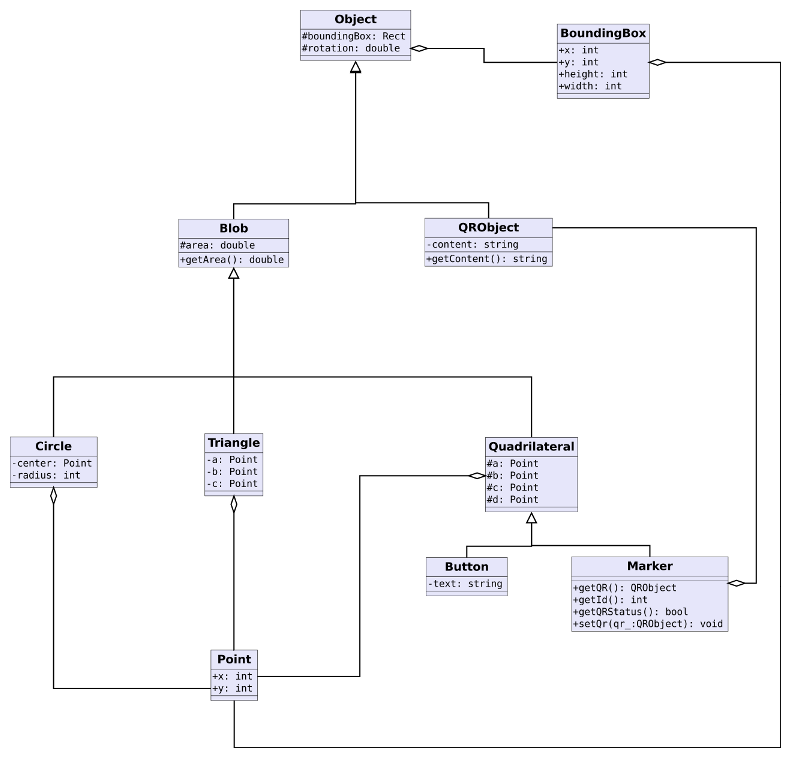
\includegraphics[scale=0.65]{images/ch_05/hierarchy.png}
	    }
	  \end{center} 
	  \caption{\textit{Class diagram illustrating the class hierarchy of the recognized objects}}  
	  \label{fig:HierarchyDesign}
 	\end{figure}

	Figure \ref{fig:HierarchyDesign} contains a class diagrams that specifies such hierarchy. 
\begin{comment}
	\emph{Object} is the superclass that represents all the possible objects recognized in an image during the feature extraction process. All the elements of this type must have a rotation value and a bounding box. The two attributes of the class \emph{rotation} and \emph{boundingBox} define such parameters. In particular, the second one has its correspondent class, called \emph{BoundingBox}. As specified in the diagram, this object can be only of rectangular shape, in fact its attributes are the coordinate of a point and horizontal and vertical dimensions.
\end{comment}
	\emph{Object} is the superclass that represents all the possible objects recognized in an image during the feature extraction process. Two attributes all the elements of this type must have are a \emph{rotation} value and a 
\emph{boundingBox}. 
	This latter parameter has a data type which is defined by the class \emph{BoundingBox}. Such element can have only rectangular shape, in fact its attributes are the coordinates of a point and horizontal and vertical dimensions.


	The type Object can be specified by two sub-types: \emph{Blob}, that represents a generic shape, and \emph{QR}, representing a \mbox{QR} element. The presence of \mbox{QR} is not important for the shape recognition task but it justifies the presence of Blob in the hierarchy. Without \mbox{QR} class, in fact, Blob could have been incorporated in Object.
	Blob is provided of the attributes \emph{area} and \emph{perimeter}, which, as suggested by the names, represent respectively the area and the perimeter of the shape.
	

	The classes \emph{Circle}, \emph{Triangle} and \emph{Quadrilateral} extend \emph{Blob}. They represent the simple shapes that can be recognized during the recognition process. Each item is defined starting by basic geometrical elements: the circle by center and radius, the triangle by three points, the quadrilateral by four points. \emph{Point} class, in particular, has been introduced in this diagram for reasons of completeness. 

	The class \emph{Button} specifies Quadrilateral by adding the attribute \emph{text}, which represents the message of such button. The fact that such class derives Quadrilateral instead of Blob reflects the requirement that the buttons can be only rectangular. 
	
	The class \emph{Marker} is not described in this document. You can find the motivation of this choice at the beginning of this chapter.


	\section{Flexibility of the design}			
	This section explains why the team designed at the beginning of the project a reference structure for the class hierarchy and the feature extraction. The two main motivations are: well defined requirements and high flexibility of such design. %The requirements are described in chapter \ref{chObjective}. Below it is discussed about such flexibility.
	
	The requirements in chapter \ref{chObjective} define precisely which are the objects, the shapes and the other features to be recognized in the images.

	The design of the class hierarchy and the feature extraction part guarantees a flexibility that allows the developers to add transparently many kind of different objects to it and introduce new features to be recognized.
	Adding further simple shapes to the hierarchy, for example, it is a task that can be accomplished easily by deriving a new type by Blob. This operation does not need to change the interface of no one of the existing classes.
	In the same way, a completely new category of object can be added simply by deriving it from Object, again without changing anything in the other classes. 
	Even the introduction of the recognition of a new feature is transparent in this architecture. It is sufficient to add a method in the FeatureExtractor class and the correspondent object, or parameter, in the hierarchy. If objects of such new kind are recognized in an image, they are added to the object list by FeatureExtractor. So nothing changes for all the other classes.

	The flexibility guaranteed by these two models allowed the developers to specify their design at the beginning of the development process.

\begin{comment} 
	
	
	\section{Communication with ACT-R}

  
  \section{The Whole Software}
  The aim of the 
  \begin{figure}[h]
	  \begin{center} 
		%TODO: aggiungere immagine	
	    %\includegraphics[scale=0.1]{images/ch_04/classDesign.jpg}
	  \end{center} 
	  \caption{\textit{Class diagram of the whole software }}  
	  \label{fig:swArchitecture}
  \end{figure}
  \todo{cambiare l immagine e aggiungere la descrizione...}.

  
  \section{The Class Hierarchy}
  \begin{figure}[h]
	  \begin{center} 
		%TODO: aggiungere immagine
	    %\includegraphics[scale=0.2]{images/ch_04/designClassObjectHierarchy.jpeg}
	  \end{center} 
	  \caption{\textit{Class hierarchy of the recognized objects}}  
	  \label{fig:callHierarchy}
  \end{figure}
   {\newpage}
   {\newpage}
   {\newpage}
   {\newpage}
  The picture above describes the hierarchy of the classes defined to contain the objects detected in the images. The \textit{Object} class represents a generic object that can be found in an image. Thus, everything which is different from the background can be seen as an instance of the \textit{Object} class. Every object must be bounded by a \textit{bounding box}. This structure is represented by the \textit{BoundingBox} class. All the bounding boxes have rectangular shape. The requirements were such that it was not necessary to define more complicate shapes \todo{migliorare questa frase, fa schifo}. The \textit{attended} attribute of the \textit{Object}  class is set to \textit{true} if the object has been already returned to ACT-R, otherwise it is set to \textit{false}. The \textit{rotation} is a value that gives the amount of the rotation in the counterclockwise directions starting from the horizontal direction \todo{controllare la correttezza}. \todo{vedere se il metodo getChunk esiste ancora}\todo{se 
non esiste eliminarlo 
dall immagine}.
  Besides the generic objects, there are two categories of object that can be found in the processed images, the \textit{QR codes} and the \textit{simples shapes}. A simple shape can be, for example, a circle, a square, a rectangle or a triangle. The QR codes is represented in the hierarchy with the \textit{QRObject} class, the generic shape with the \textit{Blob} class.
  This class has the \textit{area} parameter, which stands for the area of the object in pixel, and the  \textit{getArea} method, which returns this value. The \textit{Blob} class is realized by three classes, \textit{Circle}, \textit{Triangle} and \textit{Quadrilateral}. 
  The first one has, as parameters, the \textit{center} and the \textit{radius} of the circle itself.
  The parameters of the \textit{Triangle} and the \textit{Quadrilateral} classes are respectively three and four points, which represent the vertices of the shape. Notice that the \textit{Quadrilateral} class defines every polygon with four sides and four vertices. Thus, rectangles and squares can be instances of this class. 
  The \textit{Button} class is a realization of the \textit{Quadrilateral} class. This is because, as a requirement, buttons have always rectangular or squared shapes. The additional information they add is the \textit{text}, that is a simple message that is always present in a button. It is represented by the \textit{text} attribute. 
  The \textit{Point} class identifies a generic point in the bidimensional space. Its parameters, \textit{x} and \textit{y}, are the two coordinates in the plane.
 
  \todo{... aggiungere, correggere o finire}

  
 \end{comment} 
  
  
  
